\documentclass[tikz,border=20pt]{standalone}
\usepackage{tikz}
\usepackage{amsmath}
\usetikzlibrary{matrix,fit,backgrounds,calc,positioning}

\begin{document}
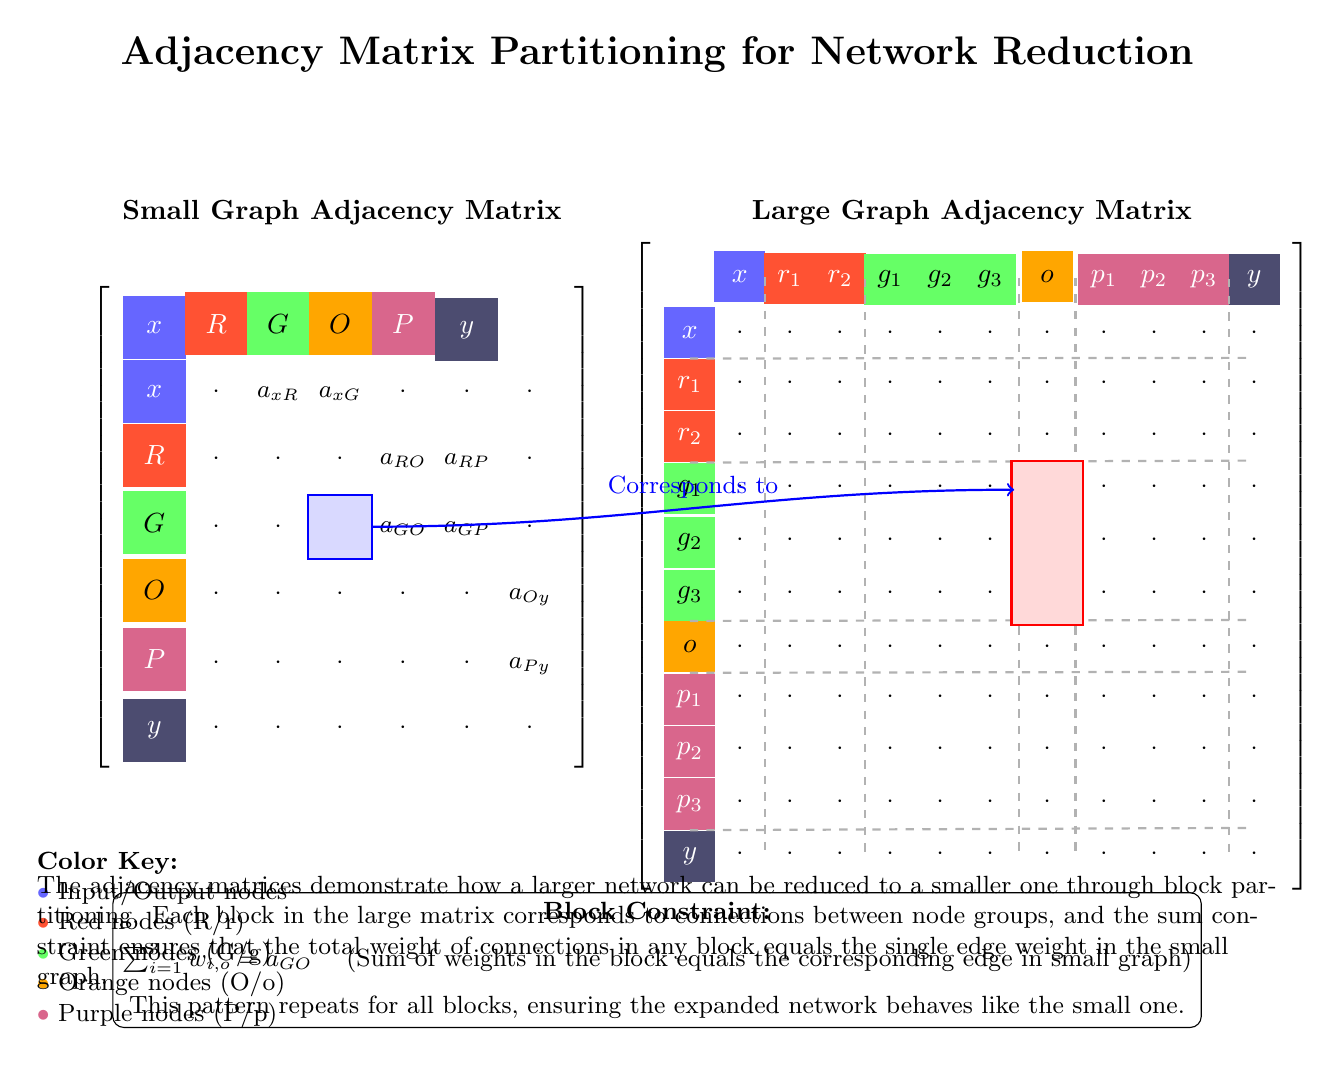
\begin{tikzpicture}[
    % Node styles
    smallmatrix/.style={
        matrix of nodes,
        nodes={minimum size=0.8cm, font=\small},
        row sep=-\pgflinewidth,
        column sep=-\pgflinewidth,
        nodes in empty cells,
        left delimiter={[},
        right delimiter={]},
    },
    largematrix/.style={
        matrix of nodes,
        nodes={minimum size=0.65cm, font=\small},
        row sep=-\pgflinewidth,
        column sep=-\pgflinewidth,
        nodes in empty cells,
        left delimiter={[},
        right delimiter={]},
    },
    hlcell/.style={fill=blue!15, draw=blue, thick, inner sep=0pt},
    hlblock/.style={fill=red!15, draw=red, thick, inner sep=1pt},
    xnode/.style={fill=blue!60, text=white, font=\bfseries},
    ynode/.style={fill=blue!20!black!70, text=white, font=\bfseries},
    rnode/.style={fill=red!70!orange!80, text=white, font=\bfseries},
    gnode/.style={fill=green!60, text=black, font=\bfseries},
    onode/.style={fill=orange!70!yellow, text=black, font=\bfseries},
    pnode/.style={fill=purple!60, text=white, font=\bfseries},
]

% Small graph adjacency matrix
\node[font=\bfseries] at (-4,4) {Small Graph Adjacency Matrix};

\matrix (SmallMatrix) [smallmatrix] at (-4,0) {
|[xnode]| $x$ & |[rnode]| $R$ & |[gnode]| $G$ & |[onode]| $O$ & |[pnode]| $P$ & |[ynode]| $y$ \\
|[xnode]| $x$ & $\cdot$ & $a_{xR}$ & $a_{xG}$ & $\cdot$ & $\cdot$ & $\cdot$ \\
|[rnode]| $R$ & $\cdot$ & $\cdot$ & $\cdot$ & $a_{RO}$ & $a_{RP}$ & $\cdot$ \\
|[gnode]| $G$ & $\cdot$ & $\cdot$ & $\cdot$ & $a_{GO}$ & $a_{GP}$ & $\cdot$ \\
|[onode]| $O$ & $\cdot$ & $\cdot$ & $\cdot$ & $\cdot$ & $\cdot$ & $a_{Oy}$ \\
|[pnode]| $P$ & $\cdot$ & $\cdot$ & $\cdot$ & $\cdot$ & $\cdot$ & $a_{Py}$ \\
|[ynode]| $y$ & $\cdot$ & $\cdot$ & $\cdot$ & $\cdot$ & $\cdot$ & $\cdot$ \\
};

% Highlight one edge in the small matrix
\node[hlcell, fit=(SmallMatrix-4-4)] {};

% Large graph adjacency matrix with improved structure
\node[font=\bfseries] at (4,4) {Large Graph Adjacency Matrix};

\matrix (LargeMatrix) [largematrix] at (4,-0.5) {
 & |[xnode]| $x$ & |[rnode]| $r_1$ & |[rnode]| $r_2$ & |[gnode]| $g_1$ & |[gnode]| $g_2$ & |[gnode]| $g_3$ & |[onode]| $o$ & |[pnode]| $p_1$ & |[pnode]| $p_2$ & |[pnode]| $p_3$ & |[ynode]| $y$ \\
|[xnode]| $x$ & $\cdot$ & $\cdot$ & $\cdot$ & $\cdot$ & $\cdot$ & $\cdot$ & $\cdot$ & $\cdot$ & $\cdot$ & $\cdot$ & $\cdot$ \\
|[rnode]| $r_1$ & $\cdot$ & $\cdot$ & $\cdot$ & $\cdot$ & $\cdot$ & $\cdot$ & $\cdot$ & $\cdot$ & $\cdot$ & $\cdot$ & $\cdot$ \\
|[rnode]| $r_2$ & $\cdot$ & $\cdot$ & $\cdot$ & $\cdot$ & $\cdot$ & $\cdot$ & $\cdot$ & $\cdot$ & $\cdot$ & $\cdot$ & $\cdot$ \\
|[gnode]| $g_1$ & $\cdot$ & $\cdot$ & $\cdot$ & $\cdot$ & $\cdot$ & $\cdot$ & $w_{1,o}$ & $\cdot$ & $\cdot$ & $\cdot$ & $\cdot$ \\
|[gnode]| $g_2$ & $\cdot$ & $\cdot$ & $\cdot$ & $\cdot$ & $\cdot$ & $\cdot$ & $w_{2,o}$ & $\cdot$ & $\cdot$ & $\cdot$ & $\cdot$ \\
|[gnode]| $g_3$ & $\cdot$ & $\cdot$ & $\cdot$ & $\cdot$ & $\cdot$ & $\cdot$ & $w_{3,o}$ & $\cdot$ & $\cdot$ & $\cdot$ & $\cdot$ \\
|[onode]| $o$ & $\cdot$ & $\cdot$ & $\cdot$ & $\cdot$ & $\cdot$ & $\cdot$ & $\cdot$ & $\cdot$ & $\cdot$ & $\cdot$ & $\cdot$ \\
|[pnode]| $p_1$ & $\cdot$ & $\cdot$ & $\cdot$ & $\cdot$ & $\cdot$ & $\cdot$ & $\cdot$ & $\cdot$ & $\cdot$ & $\cdot$ & $\cdot$ \\
|[pnode]| $p_2$ & $\cdot$ & $\cdot$ & $\cdot$ & $\cdot$ & $\cdot$ & $\cdot$ & $\cdot$ & $\cdot$ & $\cdot$ & $\cdot$ & $\cdot$ \\
|[pnode]| $p_3$ & $\cdot$ & $\cdot$ & $\cdot$ & $\cdot$ & $\cdot$ & $\cdot$ & $\cdot$ & $\cdot$ & $\cdot$ & $\cdot$ & $\cdot$ \\
|[ynode]| $y$ & $\cdot$ & $\cdot$ & $\cdot$ & $\cdot$ & $\cdot$ & $\cdot$ & $\cdot$ & $\cdot$ & $\cdot$ & $\cdot$ & $\cdot$ \\
};

% Add block separators - vertical
\draw[dashed, gray!60, thick] ($(LargeMatrix-1-2)!0.5!(LargeMatrix-1-3)$) -- ($(LargeMatrix-12-2)!0.5!(LargeMatrix-12-3)$);
\draw[dashed, gray!60, thick] ($(LargeMatrix-1-4)!0.5!(LargeMatrix-1-5)$) -- ($(LargeMatrix-12-4)!0.5!(LargeMatrix-12-5)$);
\draw[dashed, gray!60, thick] ($(LargeMatrix-1-7)!0.5!(LargeMatrix-1-8)$) -- ($(LargeMatrix-12-7)!0.5!(LargeMatrix-12-8)$);
\draw[dashed, gray!60, thick] ($(LargeMatrix-1-8)!0.5!(LargeMatrix-1-9)$) -- ($(LargeMatrix-12-8)!0.5!(LargeMatrix-12-9)$);
\draw[dashed, gray!60, thick] ($(LargeMatrix-1-11)!0.5!(LargeMatrix-1-12)$) -- ($(LargeMatrix-12-11)!0.5!(LargeMatrix-12-12)$);

% Add block separators - horizontal
\draw[dashed, gray!60, thick] ($(LargeMatrix-2-1)!0.5!(LargeMatrix-3-1)$) -- ($(LargeMatrix-2-12)!0.5!(LargeMatrix-3-12)$);
\draw[dashed, gray!60, thick] ($(LargeMatrix-4-1)!0.5!(LargeMatrix-5-1)$) -- ($(LargeMatrix-4-12)!0.5!(LargeMatrix-5-12)$);
\draw[dashed, gray!60, thick] ($(LargeMatrix-7-1)!0.5!(LargeMatrix-8-1)$) -- ($(LargeMatrix-7-12)!0.5!(LargeMatrix-8-12)$);
\draw[dashed, gray!60, thick] ($(LargeMatrix-8-1)!0.5!(LargeMatrix-9-1)$) -- ($(LargeMatrix-8-12)!0.5!(LargeMatrix-9-12)$);
\draw[dashed, gray!60, thick] ($(LargeMatrix-11-1)!0.5!(LargeMatrix-12-1)$) -- ($(LargeMatrix-11-12)!0.5!(LargeMatrix-12-12)$);

% Highlight the G to O block
\node[hlblock, fit=(LargeMatrix-5-8)(LargeMatrix-7-8)] {};

% Clean central constraint box
\node[draw, rounded corners, fill=white, align=center, font=\small, minimum width=9cm] at (0,-5.5) {
    \textbf{Block Constraint:}\\[6pt]
    $\sum_{i=1}^{3} w_{i,o} = a_{GO}$ \quad (Sum of weights in the block equals the corresponding edge in small graph)\\[6pt]
    This pattern repeats for all blocks, ensuring the expanded network behaves like the small one.
};

% Add arrow connecting the highlighted elements
\draw[->, thick, blue] (SmallMatrix-4-4) to[out=0, in=180] 
    node[midway, above, font=\small] {Corresponds to} 
    (LargeMatrix-5-8);

% Title for the overall diagram
\node[font=\Large\bfseries] at (0,6) {Adjacency Matrix Partitioning for Network Reduction};

% Explanation of colors
\node[align=left, anchor=north west, font=\small] at (-8,-4) {
    \textbf{Color Key:}\\
    \textcolor{blue!60}{$\bullet$} Input/Output nodes\\
    \textcolor{red!70!orange!80}{$\bullet$} Red nodes (R/r)\\
    \textcolor{green!60}{$\bullet$} Green nodes (G/g)\\
    \textcolor{orange!70!yellow}{$\bullet$} Orange nodes (O/o)\\
    \textcolor{purple!60}{$\bullet$} Purple nodes (P/p)
};

% Additional explanation
\node[align=left, anchor=south west, font=\small, text width=16cm] at (-8,-6) {
    The adjacency matrices demonstrate how a larger network can be reduced to a smaller one through block partitioning.
    Each block in the large matrix corresponds to connections between node groups, and the sum constraint
    ensures that the total weight of connections in any block equals the single edge weight in the small graph.
};

\end{tikzpicture}
\end{document}